\section{Outlook of the technology}
% (provide a snapshot of the main characteristics/functionality of the technology described in this lab script)

\subsection{Setup/Installation (SW/HW)}
% (describe the way to start using the technology, namely the setpup/installation SW/HW requirements, operating systems, development platforms,…)

\subsubsection{Windows Setup}
To start the lab script, students must ensure their Windows workstations meet the following requirements:

Hardware Requirements:
\begin{itemize}
    \item A personal computer (desktop or laptop).
    \item A video camera (built-in or USB peripheral).
    \item An active connection to a Local Area Network (LAN), either via Wi-Fi or an Ethernet cable.
\end{itemize}

Software and Development Platform Requirements:
\begin{itemize}
    \item Operating System: Microsoft Windows (Windows 10 or 11 is recommended).
    \item Platform: Python 3.8 (or higher) installed. During the installation process, it is strictly necessary to check the "Add Python to PATH" option to allow the execution of global commands, as shown in Figure \ref{fig:python_path}.
    
    \begin{figure}[h]
        \centering
        % Aqui o LaTeX vai buscar a tua primeira imagem!
        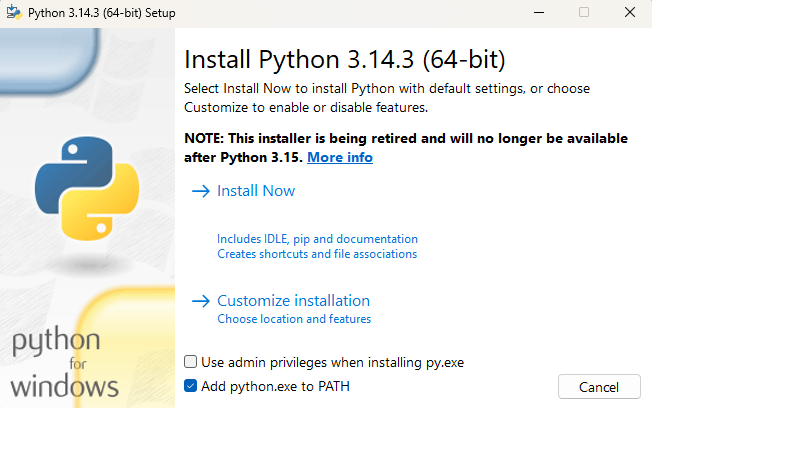
\includegraphics[width=0.6\textwidth]{imagens/python.png}
        \caption{Adding Python to PATH during installation.}
        \label{fig:python_path}
    \end{figure}

    \item Environment: An Integrated Development Environment (IDE) such as Visual Studio Code (VS Code) is recommended.
    \item Dependencies: The computer vision libraries must be installed via the Windows Command Prompt (\texttt{cmd}) or PowerShell. The student must execute the following command using the \texttt{pip} package manager, as demonstrated in Figure \ref{fig:cmd_pip}:
    
    \begin{figure}[h]
        \centering
        % Aqui o LaTeX vai buscar a tua segunda imagem!
        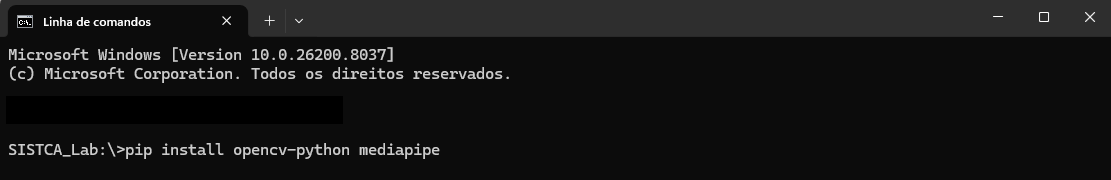
\includegraphics[width=0.8\textwidth]{imagens/cmd.png}
        \caption{Installing required libraries via Command Prompt.}
        \label{fig:cmd_pip}
    \end{figure}
\end{itemize}

\subsubsection{Linux Setup}
If you are using Linux we'll assume you have a basic understanding of the command line and already have Visual Studio Code installed, so you can follow these steps to set up your environment:
\begin{enumerate}
    \item Choose or create the directory where you want to create your project.
    \item Open a terminal and make sure your system is up to date by running:
    \begin{lstlisting}[language=bash]
# Linux Update Commands
@sudo@ apt update
@sudo@ apt upgrade
    \end{lstlisting}
    \item Install Python and pip if you haven't already:
    \begin{lstlisting}[language=bash]
# Linux Python Installation Commands
@sudo@ apt install python3 python3-pip python3-venv
    \end{lstlisting}
    \item Inside your project directory, open a terminal and create a virtual environment for your project (optional but recommended):
    \begin{lstlisting}[language=bash, ]
# Linux Virtual Environment Commands
@python3@ -m venv myvenv
@source@ myvenv/bin/activate
    \end{lstlisting}
    \item \sloppy Inside Visual Studio Code (\textit{in your project directory}), open the Command Palette (Ctrl+Shift+P) and select ``Python: Select Interpreter''. Choose the interpreter from your virtual environment (it should be something like \textbf{`myvenv/bin/python`}).
    \item Upgrage pip and install the following packages:
    \begin{lstlisting}[language=bash]
# Linux Package Installation Commands
@pip@ install --upgrade pip
@pip@ install opencv-python mediapipe scikit-learn pandas
    \end{lstlisting}
\end{enumerate}


\subsection{First Steps}

The development of the Hand-Tracking Software begins with the use of the \textbf{OpenCV} library alongside the front-facing camera to obtain a video feed in real-time, aiming to continuously capture hand movements and gestures.

The function \verb|cap = cv2.VideoCapture(n)| is responsible for the camera initialization. The index $n=0$ refers to built-in webcams commonly found in laptops, whereas higher indexes ($n=1,2,...$) allow access to secondary cameras connected via USB. It's crucial for both the camera and processor to capture the images at a high framerate to ensure smooth hand tracking and increased precision for analysis.

Before sending the image to the algorithm, pre-processing is required. OpenCV captures frames in the \textbf{BGR} format (Blue, Green, Red). The function \verb|cv2.cvtColor(frame, cv2.COLOR_BGR2RGB)| will convert it to the \textbf{RGB} format (Red, Green, Blue), which is the standard format used by most Deep Learning Models to ensure correct Inference (AI Processing). In addition, mirroring the frame with the function \verb|cv2.flip(frame, 1)| provides a more intuitive feed for the user.

\begin{lstlisting}[title={Basic Camera Feed using OpenCV}, language=Python, captionpos=b]
import cv2

cap = cv2.VideoCapture(0)
cv2.namedWindow('Hand Tracker', cv2.WINDOW_NORMAL)

while True:
    ret, frame = cap.read()
    if not ret:
        print("Error: Failed to grab frame.")
        break
 
    frame = cv2.flip(frame, 1)
    rgb_frame = cv2.cvtColor(frame, cv2.COLOR_BGR2RGB)

    cv2.imshow('Hand Tracker', frame)
    if cv2.waitKey(1) & 0xFF == ord('q'):
        break

cap.release()
cv2.destroyAllWindows()
\end{lstlisting}

The next step is to pass the frames through the MediaPipe model, which analyses the image and returns 21 Hand Landmarks placed throughout the hand, storing their respective coordinates. The analysis is triggered by calling the function \verb|results = hands.process(rgb_frame)|. Following the Inference, if a hand is detected, the coordinates are connected by lines and drawn onto the original frame, which is then displayed in the window feed.

\begin{lstlisting}[title={Mediapipe Frame Analysis}, language=Python, captionpos=b]
import cv2
import mediapipe as mp

# MediaPipe Model Config
mp_hands = mp.solutions.hands
mp_drawing = mp.solutions.drawing_utils
hands = mp_hands.Hands(min_detection_confidence=0.9, min_tracking_confidence=0.9)

# MediaPipe Coordinates to Finger Tip ID (Index, Middle, Ring, Pinky)
finger_tips = [8, 12, 16, 20]
thumb_tip = 4

# OpenCV Camera Feed
cap = cv2.VideoCapture(0)

while cap.isOpened():
    ret, frame = cap.read()
    if not ret: break
    
    frame = cv2.flip(frame, 1)
    rgb_frame = cv2.cvtColor(frame, cv2.COLOR_BGR2RGB)
    results = hands.process(rgb_frame)

    if results.multi_hand_landmarks:
        # We use 'enumerate' to know which hand we're looking at
        for hand_idx, hand_landmarks in enumerate(results.multi_hand_landmarks):
            
            # Draw Lines and Coordinates in Hand
            mp_drawing.draw_landmarks(frame, hand_landmarks, mp_hands.HAND_CONNECTIONS)

            # Find which hand (left or right) is being detected
            hand_label = results.multi_handedness[hand_idx].classification[0].label
            raised_fingers = 0

            # 1. Thumb Logic (X-Axis)
            if hand_label == "Right":
                if hand_landmarks.landmark[thumb_tip].x < hand_landmarks.landmark[thumb_tip - 1].x:
                    raised_fingers += 1
            else: # "Left"
                if hand_landmarks.landmark[thumb_tip].x > hand_landmarks.landmark[thumb_tip - 1].x:
                    raised_fingers += 1

            # 2. Other 4 Fingers Logic (Y-Axis)
            for tip in finger_tips:
                # On the Window, the Y-Axis increases downward
                if hand_landmarks.landmark[tip].y < hand_landmarks.landmark[tip - 2].y:
                    raised_fingers += 1

            # Write Text in Window
            cv2.putText(frame, f'{hand_label} hand: {raised_fingers} fingers', 
                       (10, 50 + (hand_idx * 50)),
                       cv2.FONT_HERSHEY_SIMPLEX, 1, (0, 255, 0), 2, cv2.LINE_AA)

    cv2.imshow('Hand Tracker', frame)
    if cv2.waitKey(1) & 0xFF == ord('q'): break

cap.release()
cv2.destroyAllWindows()
\end{lstlisting}

This continuous cycle of frame acquisition and immediate algorithmic analysis makes up the fundamental core of this project. The following chapter will elaborate on how the 21 hand landmarks can be used to detect patterns and movements. By leveraging this data, we can send commands to the computer, enabling control over the system through hand gestures alone.